%%%%%%%%%%%%%%%%%%%%%%%%%%%%%%%%%%%%%
% Tracing Overhead
%%%%%%%%%%%%%%%%%%%%%%%%%%%%%%%%%%%%%


\subsection{Tracing overhead}
\label{subsec:lowtoh}

 
% ORIGINAL TABLE
\iffalse
\begin{table}[]
\caption{Overhead added by each tool. Last column is the geometric mean}
\label{comet_sd_pMpAcg_BC_itn_p3.5}\begin{center}
\npdecimalsign{.}
\nprounddigits{1}
\begin{tabular}{lrrrrrrrrr}
\hline
                &   bt &   cg &    ep &    ft &   is &   lu &   mg &   sp &   GM \\
\hline
 pinMain.B.1    & 1.55 & 1.82 &  2.62 &  2.11 & 2.47 & 1.31 & 2.53 & 1.33 & 1.90 \\
 pinMain.B.4    & 1.76 & 1.85 &  1.89 &  1.74 & 1.78 & 1.77 & 1.52 & 1.73 & 1.75 \\
 pinMain.B.16   & 2.15 & 2.58 &  1.99 &  1.89 & 1.78 & 2.73 & 2.43 & 2.15 & 2.19 \\
 pinMain.B.64   & 2.10 & 2.17 &  2.39 &  1.96 & 4.31 & 4.39 & 1.97 & 2.07 & 2.52 \\
 AVG            & 1.89 & 2.10 &  2.22 &  1.92 & 2.58 & 2.55 & 2.11 & 1.82 & 2.09 \\
 pinAll.B.1     & 1.84 & 2.73 &  4.18 &  2.78 & 4.22 & 1.73 & 4.75 & 1.72 & 2.77 \\
 pinAll.B.4     & 2.57 & 3.06 &  3.41 &  2.77 & 2.96 & 2.76 & 2.79 & 2.66 & 2.86 \\
 pinAll.B.16    & 3.52 & 4.20 &  3.39 &  2.94 & 2.83 & 4.30 & 4.46 & 3.65 & 3.62 \\
 pinAll.B.64    & 3.14 & 3.26 &  3.83 &  3.02 & 5.44 & 4.65 & 3.17 & 3.31 & 3.65 \\
 AVG            & 2.77 & 3.31 &  3.70 &  2.88 & 3.86 & 3.36 & 3.79 & 2.83 & 3.23 \\
 callgrind.B.1  & 8.62 & 5.96 &  8.92 & 10.14 & 2.52 & 7.54 & 3.27 & 6.61 & 6.10 \\
 callgrind.B.4  & 6.02 & 3.60 &  2.90 &  3.50 & 1.46 & 5.18 & 1.24 & 5.78 & 3.23 \\
 callgrind.B.16 & 4.28 & 3.26 &  2.24 &  2.17 & 1.70 & 4.62 & 1.81 & 4.34 & 2.84 \\
 callgrind.B.64 & 2.26 & 2.03 &  1.66 &  2.05 & 4.07 & 3.97 & 1.47 & 2.46 & 2.34 \\
 AVG            & 5.29 & 3.71 &  3.93 &  4.46 & 2.44 & 5.33 & 1.95 & 4.80 & 3.63 \\
 pinMain.C.1    & 1.41 & 1.29 &  2.51 &  1.89 & 2.29 & 1.12 & 1.74 & 1.10 & 1.60 \\
 pinMain.C.4    & 1.58 & 1.73 &  1.75 &  1.62 & 1.68 & 1.33 & 1.81 & 1.35 & 1.60 \\
 pinMain.C.16   & 1.82 & 2.38 &  2.46 &  1.51 & 1.80 & 2.18 & 2.36 & 1.80 & 2.01 \\
 pinMain.C.64   & 2.23 & 2.74 &  2.39 &  1.59 & 4.46 & 3.42 & 2.43 & 2.24 & 2.57 \\
 AVG            & 1.76 & 2.04 &  2.28 &  1.65 & 2.56 & 2.01 & 2.08 & 1.62 & 1.94 \\
 pinAll.C.1     & 1.47 & 1.55 &  3.17 &  1.97 & 2.82 & 1.23 & 2.52 & 1.19 & 1.87 \\
 pinAll.C.4     & 1.89 & 2.42 &  2.56 &  2.06 & 2.56 & 1.70 & 3.08 & 1.71 & 2.20 \\
 pinAll.C.16    & 2.69 & 3.47 &  4.07 &  2.14 & 2.80 & 3.18 & 3.98 & 2.54 & 3.04 \\
 pinAll.C.64    & 3.61 & 4.13 &  4.21 &  2.22 & 5.47 & 4.43 & 4.23 & 3.02 & 3.80 \\
 AVG            & 2.42 & 2.89 &  3.50 &  2.10 & 3.41 & 2.63 & 3.45 & 2.11 & 2.73 \\
 callgrind.C.1  & 8.50 & 4.44 & 13.18 & 13.13 & 3.32 & 7.90 & 5.91 & 5.14 & 6.91 \\
 callgrind.C.4  & 8.66 & 4.46 &  4.76 &  6.37 & 1.65 & 6.38 & 2.75 & 6.34 & 4.64 \\
 callgrind.C.16 & 6.86 & 3.91 &  3.11 &  2.76 & 1.79 & 6.40 & 2.14 & 6.09 & 3.69 \\
 callgrind.C.64 & 4.37 & 3.46 &  2.13 &  2.50 & 4.24 & 5.24 & 2.08 & 3.81 & 3.30 \\
 AVG            & 7.10 & 4.07 &  5.79 &  6.19 & 2.75 & 6.48 & 3.22 & 5.34 & 4.63 \\
\hline
\end{tabular}
\npnoround
\end{center}
\end{table}
\fi



\iftrue

\begin{table}[!b]
\caption{Overhead added by each tool}
\label{comet_sd_pMpAcg_BC_itn_p3.5}\begin{center}
\npdecimalsign{.}
\nprounddigits{1}
\scalebox{0.80}{
\begin{tabular}{|c|c|c|n{2}{1}n{2}{1}n{2}{1}n{2}{1}n{2}{1}n{2}{1}n{2}{1}n{2}{1}|n{2}{1}|}
\hline
Input & Tool & \# Nodes  & \multicolumn{1}{c}{bt} & \multicolumn{1}{c}{cg} & \multicolumn{1}{c}{ep} & \multicolumn{1}{c}{ft} & \multicolumn{1}{c}{is} & \multicolumn{1}{c}{lu} & \multicolumn{1}{c}{mg} & \multicolumn{1}{c|}{sp} & \multicolumn{1}{c|}{GM} \\ \hline
\multirow{15}{*}{B} & \multirow{5}{*}{\parlotm} & 1 & 1.55 & 1.82 &  2.62 &  2.11 & 2.47 & 1.31 & 2.53 & 1.33 & 1.90 \\
 &  & 4  & 1.76 & 1.85 &  1.89 &  1.74 & 1.78 & 1.77 & 1.52 & 1.73 & 1.75 \\
 &  & 16  & 2.15 & 2.58 &  1.99 &  1.89 & 1.78 & 2.73 & 2.43 & 2.15 & 2.19 \\
 &  & 64  & 2.10 & 2.17 &  2.39 &  1.96 & 4.31 & 4.39 & 1.97 & 2.07 & 2.52 \\ \cline{3-12}
 &  & AVG & 1.89 & 2.10 &  2.22 &  1.92 & 2.58 & 2.55 & 2.11 & 1.82 & {\boldmath}2.09 \\ \cline{2-12}
 & \multirow{5}{*}{\parlota} & 1 & 1.84 & 2.73 &  4.18 &  2.78 & 4.22 & 1.73 & 4.75 & 1.72 & 2.77 \\
 & & 4     & 2.57 & 3.06 &  3.41 &  2.77 & 2.96 & 2.76 & 2.79 & 2.66 & 2.86 \\
 & & 16    & 3.52 & 4.20 &  3.39 &  2.94 & 2.83 & 4.30 & 4.46 & 3.65 & 3.62 \\
 & & 64    & 3.14 & 3.26 &  3.83 &  3.02 & 5.44 & 4.65 & 3.17 & 3.31 & 3.65 \\ \cline{3-12}
 & & AVG   & 2.77 & 3.31 &  3.70 &  2.88 & 3.86 & 3.36 & 3.79 & 2.83 & {\boldmath}3.23 \\ \cline{2-12}
 & \multirow{5}{*}{\callgrind}  & 1  & 8.62 & 5.96 &  8.92 & 10.14 & 2.52 & 7.54 & 3.27 & 6.61 & 6.10 \\
 & & 4   & 6.02 & 3.60 &  2.90 &  3.50 & 1.46 & 5.18 & 1.24 & 5.78 & 3.23 \\
 & & 16  & 4.28 & 3.26 &  2.24 &  2.17 & 1.70 & 4.62 & 1.81 & 4.34 & 2.84 \\
 & & 64  & 2.26 & 2.03 &  1.66 &  2.05 & 4.07 & 3.97 & 1.47 & 2.46 & 2.34 \\ \cline{3-12}
 & & AVG & 5.29 & 3.71 &  3.93 &  4.46 & 2.44 & 5.33 & 1.95 & 4.80 & {\boldmath}3.63 \\ \hline
 \multirow{15}{*}{C} & \multirow{5}{*}{\parlotm} & 1  & 1.41 & 1.29 &  2.51 &  1.89 & 2.29 & 1.12 & 1.74 & 1.10 & 1.60 \\
 & & 4   & 1.58 & 1.73 &  1.75 &  1.62 & 1.68 & 1.33 & 1.81 & 1.35 & 1.60 \\
 & & 16  & 1.82 & 2.38 &  2.46 &  1.51 & 1.80 & 2.18 & 2.36 & 1.80 & 2.01 \\
 & & 64  & 2.23 & 2.74 &  2.39 &  1.59 & 4.46 & 3.42 & 2.43 & 2.24 & 2.57 \\ \cline{3-12}
 & & AVG & 1.76 & 2.04 &  2.28 &  1.65 & 2.56 & 2.01 & 2.08 & 1.62 & {\boldmath}1.94 \\ \cline{2-12}
 & \multirow{5}{*}{\parlota} & 1 & 1.47 & 1.55 &  3.17 &  1.97 & 2.82 & 1.23 & 2.52 & 1.19 & 1.87 \\
 & & 4   & 1.89 & 2.42 &  2.56 &  2.06 & 2.56 & 1.70 & 3.08 & 1.71 & 2.20 \\
 & & 16  & 2.69 & 3.47 &  4.07 &  2.14 & 2.80 & 3.18 & 3.98 & 2.54 & 3.04 \\
 & & 64  & 3.61 & 4.13 &  4.21 &  2.22 & 5.47 & 4.43 & 4.23 & 3.02 & 3.80 \\ \cline{3-12}
 & & AVG & 2.42 & 2.89 &  3.50 &  2.10 & 3.41 & 2.63 & 3.45 & 2.11 & {\boldmath}2.73 \\ \cline{2-12}
 & \multirow{5}{*}{\callgrind} & 1 & 8.50 & 4.44 & 13.18 & 13.13 & 3.32 & 7.90 & 5.91 & 5.14 & 6.91 \\
 & & 4   & 8.66 & 4.46 &  4.76 &  6.37 & 1.65 & 6.38 & 2.75 & 6.34 & 4.64 \\
 & & 16  & 6.86 & 3.91 &  3.11 &  2.76 & 1.79 & 6.40 & 2.14 & 6.09 & 3.69 \\
 & & 64  & 4.37 & 3.46 &  2.13 &  2.50 & 4.24 & 5.24 & 2.08 & 3.81 & 3.30 \\ \cline{3-12}
 & & AVG & 7.10 & 4.07 &  5.79 &  6.19 & 2.75 & 6.48 & 3.22 & 5.34 & {\boldmath}4.63 \\ \hline
\end{tabular}}
\npnoround
\end{center}
\end{table}

\fi

   
Table \ref{comet_sd_pMpAcg_BC_itn_p3.5} shows the overhead caused by \parlotm, \parlota and  \callgrind on each application of NPB benchmark.
Last column of table shows the geometric mean of \textit{tracing overhead} by each tool for every application. \\
 
 

On average, both \parlotm and \parlota has better performance than \callgrind. Bolded numbers in table \ref{comet_sd_pMpAcg_BC_itn_p3.5} for input C shows that the average overhead added by \parlotm is \textbf{1.98}, by \parlota is \textbf{2.83} and by \callgrind is \textbf{4.88} (all of the overhead has been calculated relative to native run as baseline). 
\\
Considering amount of collected traces by \parlot (especially \parlota) and \callgrind, clearly \parlot reaches the goal of "collecting more while adding less overhead".
By increasing the sizes of inputs, the average of geometric means of overheads decrease for \parlotm and \parlota but increase for \callgrind. 

\begin{itemize}
\item Why Callgrind scales better? [to be added]
\item Martin's question in the email [to be added]
\item more info about type of applications that we used as benchmark and why tools have different numbers and behaviors for different applications.
\end{itemize}
 
 
\begin{figure}[!t]
\centering
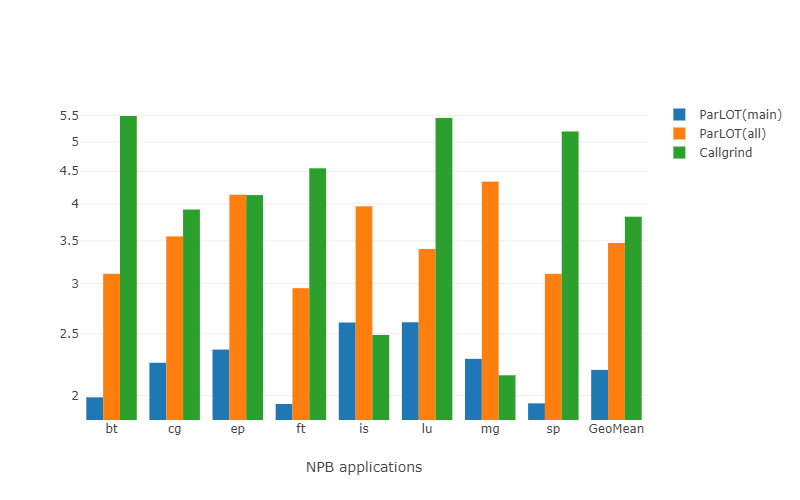
\includegraphics[width=3.9in]{figs.comet/comet_chartAvg_sd_B_p3_5.png}
\caption{ Input: \textbf{B} - Slowdown of \parlotm ,\parlota and \callgrind. Each bar is the average slowdown of each tool on each application for 1, 4 and 16 and 64 nodes (16, 64, 256 and 1024 cores). 
}
\label{comet_chartAvg_sd_B_p3_5}
\end{figure}


\begin{figure}[!t]
\centering
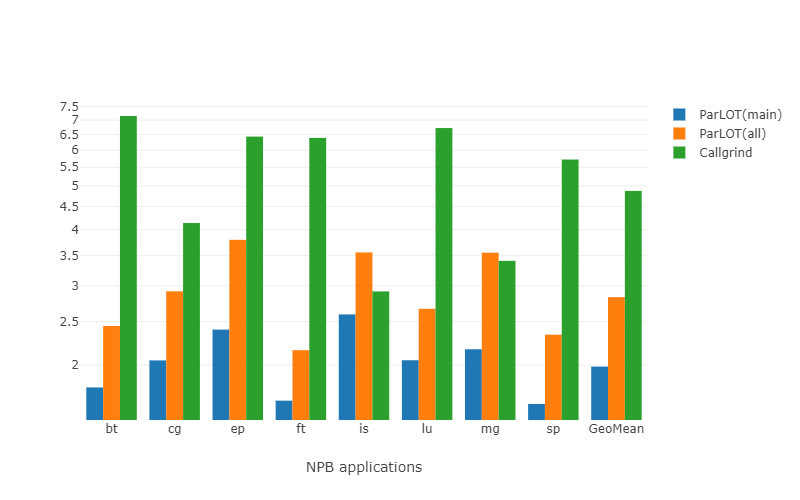
\includegraphics[width=3.9in]{figs.comet/comet_chartAvg_sd_C_p3_5.png}
\caption{ Input: \textbf{C} - Slowdown of \parlotm ,\parlota and \callgrind. Each bar is the average slowdown of each tool on each application for 1, 4 and 16 and 64 nodes (16, 64, 256 and 1024 cores). . 
}
\label{comet_chartAvg_sd_C_p3_5}
\end{figure}


 
 


%%%%%%%%%%%%%%%%%%%%%%%%%%%%%%%%%%%%%
% Banwidth
%%%%%%%%%%%%%%%%%%%%%%%%%%%%%%%%%%%%%


  
\subsection{Required Bandwidth}
\label{subsec:lowbw}
 - Table \ref{comet_bw_pMpAcg_BC_itn_p3.5}
  - Fig \ref{comet_chartAvg_bw_B_p3_5}, \ref{comet_chartAvg_bw_C_p3_5}

\begin{table*}[]
\caption{Server: \textbf{comet} - 
 Stat: \textbf{bw} - 
 Tools: pinMain , pinAll , callgrind ,  
 Inputs: B , C ,  
 Nodes: 1 , 4 , 16 , 64 ,  
 Desc: Primary
 }
\label{comet_bw_pMpAcg_BC_itn_p3.5}\begin{center}
\begin{tabular}{|l|rrrrrrrr|r|}
\hline
                &    bt &     cg &    ep &    ft &    is &     lu &    mg &     sp &    GM \\
\hline
 pinMain.B.1    &  4.72 &  21.86 &  3.83 &  1.52 &  0.79 &   2.39 &  5.62 &   5.36 &  3.69 \\
 pinMain.B.4    & 14.28 &  41.08 &  1.89 &  3.48 &  2.24 &  21.48 &  6.45 &  15.85 &  8.12 \\
 pinMain.B.16   & 14.31 &  46.59 &  1.45 &  4.86 &  3.40 &  31.79 &  6.53 &  18.55 &  9.41 \\
 pinMain.B.64   & 18.56 &  43.59 &  1.25 &  4.56 &  4.49 &  27.07 &  5.63 &  29.62 &  9.92 \\
 \hline
 AVG            & 12.97 &  38.28 &  2.10 &  3.60 &  2.73 &  20.68 &  6.06 &  17.35 &  \textbf{7.79} \\
 \hline
 pinAll.B.1     & 48.71 &  89.39 & 47.23 & 45.63 & 59.98 &  53.62 & 60.81 &  54.33 & 56.21 \\
 pinAll.B.4     & 61.84 & 101.23 & 45.21 & 55.12 & 53.20 &  71.09 & 54.85 &  73.62 & 62.68 \\
 pinAll.B.16    & 73.95 & 116.87 & 47.37 & 48.88 & 47.79 & 100.91 & 55.80 &  84.61 & 67.97 \\
 pinAll.B.64    & 81.80 & 110.15 & 44.16 & 47.98 & 37.84 & 100.26 & 52.67 &  99.90 & 66.47 \\
 \hline
 AVG            & 66.58 & 104.41 & 45.99 & 49.40 & 49.70 &  81.47 & 56.03 &  78.12 & \textbf{63.33} \\
 \hline
 callgrind.B.1  &  1.57 &   7.69 &  7.39 &  4.56 & 39.49 &   2.61 & 34.41 &   2.71 &  6.67 \\
 callgrind.B.4  &  6.51 &  16.01 & 22.10 & 15.65 & 45.46 &   8.63 & 45.47 &   7.78 & 16.31 \\
 callgrind.B.16 & 17.20 &  24.62 & 37.42 & 23.84 & 29.87 &  16.23 & 51.49 &  15.81 & 24.93 \\
 callgrind.B.64 & 26.82 &  27.65 & 45.93 & 25.14 & 11.04 &  17.75 & 45.27 &  20.20 & 25.02 \\
 \hline
 AVG            & 13.03 &  18.99 & 28.21 & 17.30 & 31.47 &  11.30 & 44.16 &  11.62 & \textbf{18.23} \\
 \hline
 \hline
 pinMain.C.1    &  1.82 &  16.96 &  5.15 &  1.16 &  0.69 &   0.77 &  3.56 &   1.40 &  2.17 \\
 pinMain.C.4    &  7.53 &  44.87 &  3.00 &  2.50 &  2.12 &  20.13 &  7.08 &  13.74 &  7.55 \\
 pinMain.C.16   & 16.30 &  55.04 &  1.84 &  6.10 &  3.35 &  34.09 &  7.24 &  20.68 & 10.70 \\
 pinMain.C.64   & 17.45 &  61.43 &  1.30 &  5.93 &  4.42 &  38.28 &  5.62 &  26.09 & 10.94 \\
 \hline
 AVG            & 10.77 &  44.58 &  2.82 &  3.92 &  2.65 &  23.32 &  5.88 &  15.48 &  \textbf{7.84} \\
 \hline
 pinAll.C.1     & 17.80 &  53.37 & 26.34 & 20.89 & 48.31 &  25.31 & 52.61 &  19.46 & 29.99 \\
 pinAll.C.4     & 51.78 &  95.84 & 36.80 & 43.82 & 51.40 &  58.39 & 54.18 &  65.77 & 55.15 \\
 pinAll.C.16    & 75.38 & 121.03 & 44.29 & 61.39 & 46.90 & 101.05 & 56.49 & 101.32 & 71.37 \\
 pinAll.C.64    & 80.63 & 135.19 & 43.49 & 46.28 & 37.09 & 117.87 & 54.05 &  99.02 & 68.99 \\
 \hline
 AVG            & 56.40 & 101.36 & 37.73 & 43.09 & 45.93 &  75.66 & 54.33 &  71.39 & \textbf{56.38} \\
 \hline
 callgrind.C.1  &  0.40 &   3.09 &  1.96 &  1.05 & 14.60 &   0.70 &  6.96 &   0.75 &  1.85 \\
 callgrind.C.4  &  1.78 &   8.87 &  7.74 &  4.48 & 31.74 &   2.82 & 21.03 &   2.78 &  6.41 \\
 callgrind.C.16 &  6.01 &  15.82 & 22.86 & 10.75 & 26.50 &   7.45 & 39.05 &   6.96 & 13.72 \\
 callgrind.C.64 & 14.32 &  19.56 & 35.75 & 12.17 & 11.07 &  11.86 & 40.69 &  12.83 & 17.39 \\
 \hline
 AVG            &  5.63 &  11.84 & 17.08 &  7.11 & 20.98 &   5.71 & 26.93 &   5.83 &  \textbf{9.84} \\
\hline
\end{tabular}
\end{center}
\end{table*}



Table \ref{comet_bw_pMpAcg_BC_itn_p3.5} shows the required bandwidth for each tool. 
In addition to big gap between average overhead of \parlotm and \callgrind, \parlotm also beats \callgrind in required bandwidth, especially for smaller inputs.

\begin{figure}[!t]
\centering
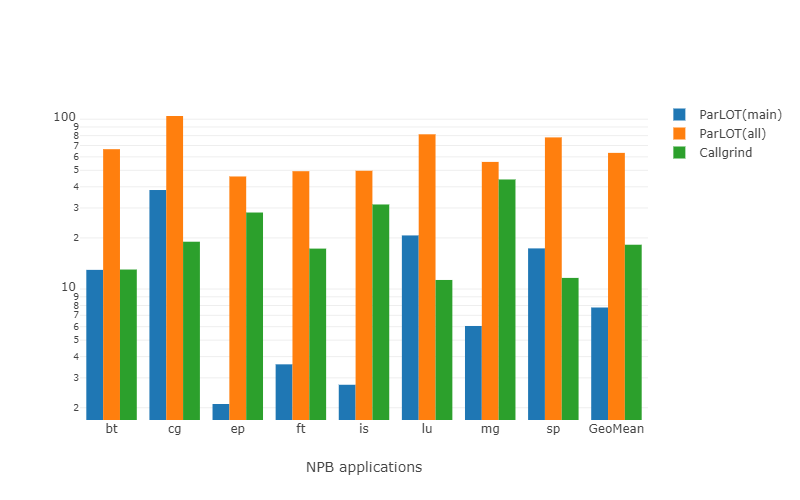
\includegraphics[width=3.5in]{figs.comet/comet_chartAvg_bw_B_p3_5.png}
\caption{ Input: \textbf{B} - Required Bandwidth per core (kB/s)
}
\label{comet_chartAvg_bw_B_p3_5}
\end{figure}


\begin{itemize}
\item 
\item According to table \ref{comet_cr_pMpA_BC_itn_p3.5}, for example for \parlota where the average compression ratio for input C is 644.38, and the correspondent required bandwidth which is 56.38, it shows that \parlot can collect almost 36 MB worth of data per core per second where it only needs 56.38 KB/S bandwidth.]
\item Low required bandwidth, low tracing overhead and high compression ratio for makes \parlot work perfect to solve the the trade-off between "more overhead to add, more information to get"
\item In addition to big gap between average overhead of \parlotm and \callgrind, \parlotm also beats \callgrind in required bandwidth, especially for smaller inputs.
	\item \textbf{\parlota vs. \callgrind}: According to table \ref{comet_cr_pMpA_BC_itn_p3.5} (from next subsection), for \parlota where the average compression ratio for input C is 644.38, and the correspondent required bandwidth which is 56.38 kB/s, it shows that \parlota can collect \textbf{more than 36 MB} worth of data per core per second where it only needs \textbf{56.38 kB/s} bandwidth, while \callgrind can only collects \textbf{less than 100 kB} of informative data and still adds more overhead comparing to either \parlota or \parlotm. \textbf{Conclusion: The amount of informative data can be collected with \parlota  are 360x larger than \callgrind and the overhead \parlota adds is less than 0.6x smaller than \callgrind}
	\item \textbf{\parlotm vs. \callgrind} Above story is true also for \parlotm. According to table \ref{comet_cr_pMpA_BC_itn_p3.5}, for \parlotm where the average compression ratio for input C is 1117.01, and the correspondent required bandwidth which is 7.84 kB/s, shows that \parlotm can collect \textbf{more than 8.5 MB} worth of data per core per second where it only needs \textbf{7.84.38 kB/s} bandwidth, while \callgrind can only collects \textbf{less than 100 kB} of informative data and still adds more overhead comparing to either \parlota or \parlotm. \textbf{Conclusion: The amount of informative data can be collected with \parlotm  are 85x larger than \callgrind and the overhead \parlotm adds is about 0.4x smaller than \callgrind}
\end{itemize}




\begin{figure}[!t]
\centering
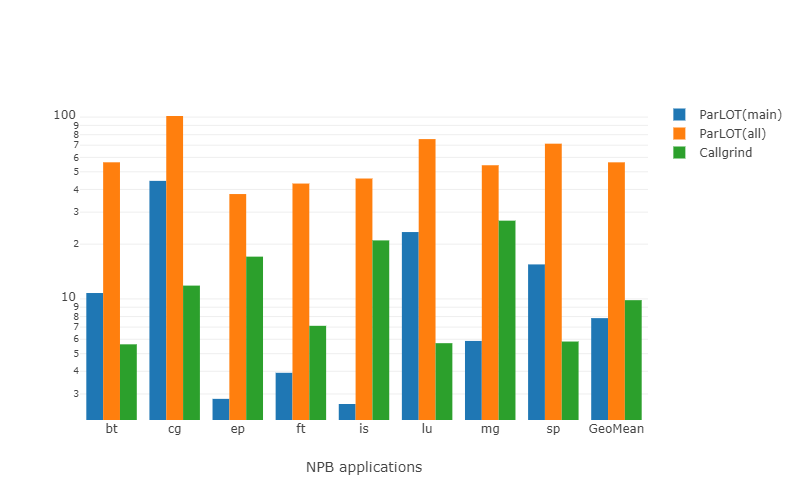
\includegraphics[width=3.5in]{figs.comet/comet_chartAvg_bw_C_p3_5.png}
\caption{ Input: \textbf{C}  - Required Bandwidth per core (kB/s)
}
\label{comet_chartAvg_bw_C_p3_5}
\end{figure}


%%%%%%%%%%%%%%%%%%%%%%%%%%%%%%%%%%%%%%%%%%%%%%%%%%%%%%%%%%%%%%%%%%%%%%%%%%%%%%%%%%
  
\subsection{Compression Ratio}
\label{subsec:cr}
 - Table \ref{comet_cr_pMpA_BC_itn_p3.5}
  - Fig \ref{comet_chartAvg_cr_B_p3_5}, \ref{comet_chartAvg_cr_C_p3_5}

  Table \ref{comet_cr_pMpA_BC_itn_p3.5} shows the compression ratios for all configs and inputs. On average, \parlot can store up to more than 1700 MB of collected data in just 1 MB trace files. Compression ratios are higher for larger input sizes (WHY?). Also \parlotm has better performance than \parlota (WHY?).
  
\textbf{Conclusion: I included some interesting facts about the charts and table of Compression ratio in previous section}
\iffalse
\begin{table}[]
\caption{Compression Ratio}
\label{comet_cr_pMpA_BC_itn_p3.5}\begin{center}
\begin{tabular}{lrrrrrrrrr}
\hline
              &      bt &     cg &       ep &       ft &       is &     lu &     mg &      sp &      GM \\
\hline
 pinMain.B.1  & 3035.93 &  94.35 & 12456.18 & 12173.49 &  9718.38 & 167.72 &  99.08 &  878.27 & 1255.17 \\
 pinMain.B.4  &  586.64 &  82.48 & 10368.41 &  1737.09 &   909.20 & 140.29 & 254.95 &  338.16 &  559.36 \\
 pinMain.B.16 &  346.66 & 113.28 &  8563.85 &  1077.35 &  1200.57 & 178.98 & 387.63 &  123.02 &  496.83 \\
 pinMain.B.64 &  252.24 & 147.78 &  7611.04 &  1122.62 &  1907.95 & 366.80 & 437.31 &  152.91 &  591.11 \\
 AVG          & 1055.37 & 109.47 &  9749.87 &  4027.64 &  3434.03 & 213.45 & 294.74 &  373.09 &  725.62 \\
 pinAll.B.1   &  514.51 & 137.41 &  3335.77 &  1226.74 &   543.18 & 314.63 & 260.87 &  303.88 &  500.21 \\
 pinAll.B.4   &  315.71 & 137.21 &  1266.92 &   436.15 &   316.16 & 287.25 & 329.57 &  199.66 &  330.70 \\
 pinAll.B.16  &  226.86 & 181.58 &  1246.66 &  1026.53 &   927.09 & 299.30 & 469.29 &  171.52 &  430.39 \\
 pinAll.B.64  &  329.23 & 247.30 &  1394.07 &  1043.94 &  1984.62 & 410.32 & 548.47 &  307.16 &  597.55 \\
 AVG          &  346.58 & 175.88 &  1810.86 &   933.34 &   942.76 & 327.88 & 402.05 &  245.56 &  464.71 \\
 pinMain.C.1  & 8618.95 & 111.16 & 13067.96 & 21335.57 & 21856.49 & 350.03 & 247.44 & 1977.43 & 2371.35 \\
 pinMain.C.4  & 1910.64 & 110.45 & 12418.66 &  6520.34 &  2256.56 & 112.77 & 267.98 &  472.68 &  928.16 \\
 pinMain.C.16 &  580.79 & 133.24 & 11017.36 &  1239.31 &  1347.88 & 164.47 & 396.86 &  143.13 &  582.78 \\
 pinMain.C.64 &  322.83 & 131.92 &  9154.99 &  1065.12 &  1896.25 & 223.69 & 465.74 &  168.89 &  585.74 \\
 AVG          & 2858.30 & 121.69 & 11414.74 &  7540.09 &  6839.30 & 212.74 & 344.50 &  690.53 & 1117.01 \\
 pinAll.C.1   & 2579.37 & 181.76 &  7376.96 &  5143.08 &  1520.42 & 408.21 & 314.77 &  650.73 & 1107.37 \\
 pinAll.C.4   &  448.61 & 161.32 &  3194.58 &  1062.94 &   527.34 & 274.70 & 319.35 &  237.43 &  477.42 \\
 pinAll.C.16  &  285.05 & 185.74 &  1765.49 &   588.86 &  1106.34 & 273.63 & 467.35 &  141.69 &  426.92 \\
 pinAll.C.64  &  290.00 & 214.68 &  1512.89 &  1237.30 &  2038.72 & 329.04 & 496.21 &  270.83 &  565.82 \\
 AVG          &  900.76 & 185.88 &  3462.48 &  2008.05 &  1298.21 & 321.39 & 399.42 &  325.17 &  644.38 \\
\hline
\end{tabular}
\end{center}
\end{table}

\fi


\iftrue

\begin{table}[]
\caption{ Compression ratio }
\label{comet_cr_pMpA_BC_itn_p3.5}\begin{center}
\npdecimalsign{.}
\nprounddigits{1}
\scalebox{0.7}{
\begin{tabular}{|c|c|c|N{5}{1}N{5}{1}N{5}{1}N{5}{1}N{5}{1}N{5}{1}n{5}{1}n{5}{1}|n{5}{1}|}
\hline
Input & Tool & \# Nodes  & \multicolumn{1}{c}{bt} & \multicolumn{1}{c}{cg} & \multicolumn{1}{c}{ep} & \multicolumn{1}{c}{ft} & \multicolumn{1}{c}{is} & \multicolumn{1}{c}{lu} & \multicolumn{1}{c}{mg} & \multicolumn{1}{c|}{sp} & \multicolumn{1}{c|}{GM} \\ \hline
\multirow{10}{*}{B} & \multirow{5}{*}{\parlotm} & 1 & 3035.93 &  94.35 & 12456.18 & 12173.49 &  9718.38 & 167.72 &  99.08 &  878.27 & 1255.17 \\
 & & 4                                               &  586.64 &  82.48 & 10368.41 &  1737.09 &   909.20 & 140.29 & 254.95 &  338.16 &  559.36 \\
 & & 16                                              &  346.66 & 113.28 &  8563.85 &  1077.35 &  1200.57 & 178.98 & 387.63 &  123.02 &  496.83 \\
 & & 64                                              &  252.24 & 147.78 &  7611.04 &  1122.62 &  1907.95 & 366.80 & 437.31 &  152.91 &  591.11 \\ \cline{3-12}
 & & AVG                                             & 1055.37 & 109.47 &  9749.87 &  4027.64 &  3434.03 & 213.45 & 294.74 &  373.09 &  {\boldmath}725.62  \\ \cline{2-12}
 & \multirow{5}{*}{\parlota} & 1 &  514.51 & 137.41 &  3335.77 &  1226.74 &   543.18 & 314.63 & 260.87 &  303.88 &  500.21 \\
 & & 4                            &  315.71 & 137.21 &  1266.92 &   436.15 &   316.16 & 287.25 & 329.57 &  199.66 &  330.70 \\
 & & 16                           &  226.86 & 181.58 &  1246.66 &  1026.53 &   927.09 & 299.30 & 469.29 &  171.52 &  430.39 \\
 & & 64                           &  329.23 & 247.30 &  1394.07 &  1043.94 &  1984.62 & 410.32 & 548.47 &  307.16 &  597.55 \\ \cline{3-12}
 & & AVG                          &  346.58 & 175.88 &  1810.86 &   933.34 &   942.76 & 327.88 & 402.05 &  245.56 &  {\boldmath}464.71 \\ \hline
 \multirow{10}{*}{C} & \multirow{5}{*}{\parlotm} & 1  & 8618.95 & 111.16 & 13067.96 & 21335.57 & 21856.49 & 350.03 & 247.44 & 1977.43 & 2371.35  \\
 & & 4                                                 & 1910.64 & 110.45 & 12418.66 &  6520.34 &  2256.56 & 112.77 & 267.98 &  472.68 &  928.16  \\
 & & 16                                                &  580.79 & 133.24 & 11017.36 &  1239.31 &  1347.88 & 164.47 & 396.86 &  143.13 &  582.78  \\
 & & 64                                                &  322.83 & 131.92 &  9154.99 &  1065.12 &  1896.25 & 223.69 & 465.74 &  168.89 &  585.74  \\ \cline{3-12}
 & & AVG                                               & 2858.30 & 121.69 & 11414.74 &  7540.09 &  6839.30 & 212.74 & 344.50 &  690.53 & {\boldmath}1117.01  \\ \cline{2-12}
 & \multirow{5}{*}{\parlota} & 1 & 2579.37 & 181.76 &  7376.96 &  5143.08 &  1520.42 & 408.21 & 314.77 &  650.73 & 1107.37 \\
 & & 4                            &  448.61 & 161.32 &  3194.58 &  1062.94 &   527.34 & 274.70 & 319.35 &  237.43 &  477.42 \\
 & & 16                           &  285.05 & 185.74 &  1765.49 &   588.86 &  1106.34 & 273.63 & 467.35 &  141.69 &  426.92 \\
 & & 64                           &  290.00 & 214.68 &  1512.89 &  1237.30 &  2038.72 & 329.04 & 496.21 &  270.83 &  565.82 \\ \cline{3-12}
 & & AVG                          &  900.76 & 185.88 &  3462.48 &  2008.05 &  1298.21 & 321.39 & 399.42 &  325.17 &  {\boldmath}644.38 \\ \cline{2-12} \hline
\end{tabular}}
\npnoround
\end{center}
\end{table}

\fi



\begin{figure}[!t]
\centering
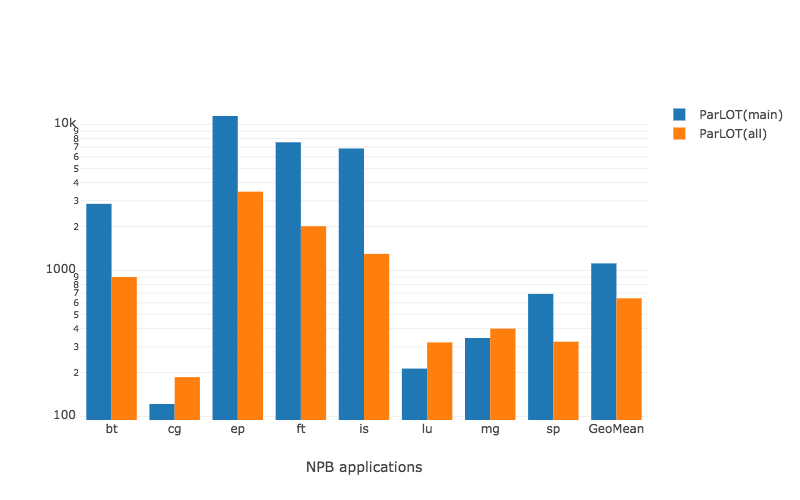
\includegraphics[width=3.5in]{figs.comet/comet_chartAvg_cr_C_p3_5.png}
\caption{ Input: \textbf{C}  - Compression Ratio
}
\label{comet_chartAvg_cr_C_p3_5}
\end{figure}


\begin{figure}[!t]
\centering
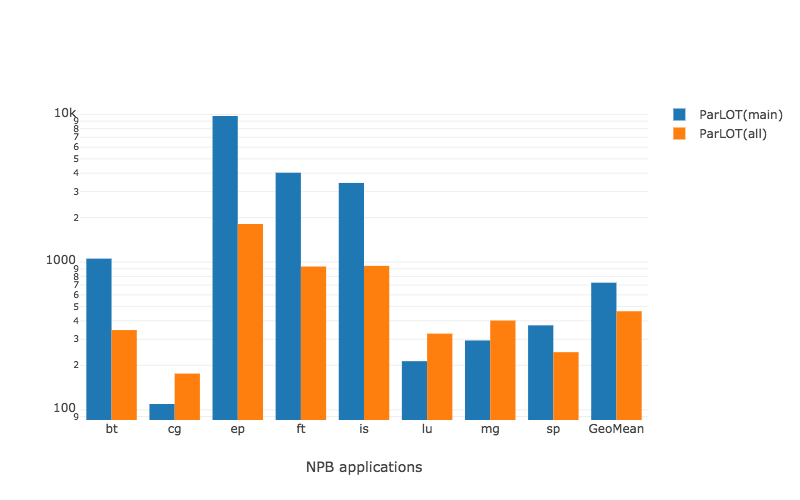
\includegraphics[width=3.5in]{figs.comet/comet_chartAvg_cr_B_p3_5.png}
\caption{ Input: \textbf{B}  - Compression Ratio
}
\label{comet_chartAvg_cr_B_p3_5}
\end{figure}
  
%%%%%%%%%%%%%%%%%%%%%%%%%%%%%%%%%%%%%%%%%%%%%%%%%%%%%%%%%%%%%  
  
\subsection{Pin-init Overhead} 
\label{subsec:pinit}
 - Table \ref{comet_wo_det_All_all_B_p3.5}, \ref{comet_wo_det_Main_all_B_p3.5}
  - Fig \ref{comet_chartDet_B_wc_byTool_p3_5}, \ref{comet_chartDet_C_wc_byTool_p3_5}
   Tables \ref{comet_wo_det_Main_all_B_p3.5}, \ref{comet_wo_det_All_all_B_p3.5} show average overhead added to each application by different variations of \parlot. Last row of tables shows geometric mean of each of its above values showing how much each phase of \parlot slows down the native execution. In general, we all expect that the added overhead of  Pin-init < \parlot < \parlotnc. Highlighted cells in tables are the ones which do not follow the above order. Number of highlighted cells for \parlot(main) is larger than \parlot(all). Variability of runtimes for \parlot(main) is more than other ones (native run, \parlot(all) and \callgrind) [new error bars to be added].
	
	\begin{itemize}
	\item \textbf{most of the added overhead by \parlot is caused by Pin-init}. According to tables \ref{comet_wo_det_Main_all_B_p3.5}, \ref{comet_wo_det_All_all_B_p3.5}, on average, Pin-init adds 3.28 overhead and \parlota adds 3.42 overhead. \textbf{almost 96\% of \parlota overhead is happening on Pin-init - Numbers from \parlotm and other inputs are following the same pattern}
	\end{itemize}
\begin{table}[]
\caption{Tracing overhead of versions of \parlotm - Input B}
\begin{center}
\label{comet_wo_det_Main_all_B_p3.5}
\scalebox{0.5}{
\begin{tabular}{|c|c|rrr|rrr|rrr|rrr|}
\hline
\multicolumn{1}{|l|}{\multirow{2}{*}{\textbf{Input: B}}} & \multicolumn{1}{r|}{Nodes :}    & \multicolumn{3}{c|}{1}  & \multicolumn{3}{c|}{4} & \multicolumn{3}{c|}{16}  & \multicolumn{3}{c|}{64} \\ \cline{2-14}
\multicolumn{1}{|l|}{} & \multicolumn{1}{r|}{Detail Tools:} & \multicolumn{1}{c}{\pininit} & \multicolumn{1}{c}{\parlot} & \multicolumn{1}{c|}{\parlotnc} & \multicolumn{1}{c}{\pininit} & \multicolumn{1}{c}{\parlot} & \multicolumn{1}{c|}{\parlotnc} & \multicolumn{1}{c}{\pininit} & \multicolumn{1}{c}{\parlot} & \multicolumn{1}{c|}{\parlotnc} & \multicolumn{1}{c}{\pininit} & \multicolumn{1}{c}{\parlot} & \multicolumn{1}{c|}{\parlotnc} \\
\hline
\multirow{9}{*}{Main} &     bt  &  1.5  &  1.5  &   5.6  &  1.7  &  1.7  &  5.0  &  2.1  &  2.1  &  5.0  &  1.8  &  2.1  &  3.5 \\
 &  cg  &  1.7  &  1.8  &   2.3  &  1.8  &  1.8  &  2.6  &  2.7  &  2.5  &  4.4  &  2.3  &  2.1  &  4.6 \\
 &  ep  &  2.9  &  2.6  &  20.4  &  1.9  &  1.8  &  5.3  &  2.4  &  1.9  &  3.0  &  2.6  &  2.3  &  2.6 \\
 &  ft  &  1.8  &  2.1  &   6.1  &  1.7  &  1.7  &  2.7  &  2.0  &  1.8  &  2.2  &  2.1  &  1.9  &  2.1 \\
 &  is  &  2.4  &  2.4  &   4.8  &  1.7  &  1.7  &  2.0  &  2.1  &  1.7  &  1.8  &  4.5  &  4.3  &  5.7 \\
 &  lu  &  1.3  &  1.3  &   1.4  &  1.7  &  1.7  &  2.2  &  2.7  &  2.7  &  3.6  &  3.0  &  4.3  &  6.1 \\
 &  mg  &  2.5  &  2.5  &   2.7  &  1.5  &  1.5  &  1.5  &  2.6  &  2.4  &  2.6  &  1.9  &  1.9  &  1.8 \\
 &  sp  &  1.3  &  1.3  &   2.4  &  1.7  &  1.7  &  3.5  &  2.1  &  2.1  &  2.3  &  1.9  &  2.0  &  2.5 \\
\cline{2-14}
 &  GM  &  1.8  &  1.9  &   4.1  &  1.7  &  1.7  &  2.9  &  2.3  &  2.1  &  3.0  &  2.4  &  2.5  &  3.3 \\
\hline
\end{tabular} }

\end{center}
\end{table}








\ignore{--
\begin{table*}[]
\caption{Tracing overhead of different \parlot versions - Input B - Main image}
\begin{center}
\label{comet_wo_det_Main_all_B_p3.5}
\scalebox{0.78}{
\begin{tabular}{|c|c|rrr|rrr|rrr|rrr|}
\hline
\multicolumn{1}{|l|}{\multirow{2}{*}{\textbf{Input: B}}} & \multicolumn{1}{r|}{Nodes :}    & \multicolumn{3}{c|}{1}  & \multicolumn{3}{c|}{4} & \multicolumn{3}{c|}{16}  & \multicolumn{3}{c|}{64} \\ \cline{2-14}
\multicolumn{1}{|l|}{} & \multicolumn{1}{r|}{Detail Tools:} & \multicolumn{1}{c}{\pininit} & \multicolumn{1}{c}{\parlot} & \multicolumn{1}{c|}{\parlotnc} & \multicolumn{1}{c}{\pininit} & \multicolumn{1}{c}{\parlot} & \multicolumn{1}{c|}{\parlotnc} & \multicolumn{1}{c}{\pininit} & \multicolumn{1}{c}{\parlot} & \multicolumn{1}{c|}{\parlotnc} & \multicolumn{1}{c}{\pininit} & \multicolumn{1}{c}{\parlot} & \multicolumn{1}{c|}{\parlotnc} \\
\hline
\multirow{9}{*}{Main} &  bt  &  1.50  &  1.55  &   5.62  &  1.74  &  1.76  &  5.06  &  2.19  &  2.15  &  5.02  &  1.83  &  2.10  &  3.52 \\
 &  cg  &  1.75  &  1.82  &   2.38  &  1.84  &  1.85  &  2.64  &  2.70  &  2.58  &  4.43  &  2.32  &  2.17  &  4.64 \\
 &  ep  &  2.96  &  2.62  &  20.48  &  1.99  &  1.89  &  5.38  &  2.47  &  1.99  &  3.09  &  2.68  &  2.39  &  2.66 \\
 &  ft  &  1.87  &  2.11  &   6.17  &  1.75  &  1.74  &  2.79  &  2.08  &  1.89  &  2.24  &  2.18  &  1.96  &  2.14 \\
 &  is  &  2.47  &  2.47  &   4.82  &  1.79  &  1.78  &  2.07  &  2.11  & 1.78  &  1.87  &  4.51  &  4.31  &  5.71 \\
 &  lu  &  1.32  &  1.31  &   1.44  &  1.75  &  1.77  &  2.25  &  2.73  &  2.73  &  3.62  &  3.05  &  4.39  &  6.13 \\
 &  mg  &  2.56  &  2.53  &   2.79  &  1.56  &  1.52  &  1.59  &  2.63  &  2.43  &  2.65  &  1.95  &  1.97  &  1.85 \\
 &  sp  &  1.34  &  1.33  &   2.43  &  1.73  &  1.73  &  3.58  &  2.14  &  2.15  &  2.37  &  1.95  &  2.07  &  2.54 \\
\cline{2-14}
 &  GM  &  1.89  &  1.90  &   4.10  &  1.77  &  1.75  &  2.92  &  2.37  &  2.19  &  3.00  &  2.45  &  2.52  &  3.33 \\
\hline
\end{tabular} }

\end{center}
\end{table*}
}


\begin{table}[]
\caption{Tracing overhead of versions of \parlota - Input B}
\begin{center}
\label{comet_wo_det_All_all_B_p3.5}
\scalebox{0.78}{
\begin{tabular}{|c|c|rrr|rrr|rrr|rrr|}
\hline
\multicolumn{1}{|l|}{\multirow{2}{*}{\textbf{Input: B}}} & \multicolumn{1}{r|}{Nodes :}    & \multicolumn{3}{c|}{1}  & \multicolumn{3}{c|}{4} & \multicolumn{3}{c|}{16}  & \multicolumn{3}{c|}{64} \\ \cline{2-14}
\multicolumn{1}{|l|}{} & \multicolumn{1}{r|}{Detail Tools:} & \multicolumn{1}{c}{\pininit} & \multicolumn{1}{c}{\parlot} & \multicolumn{1}{c|}{\parlotnc} & \multicolumn{1}{c}{\pininit} & \multicolumn{1}{c}{\parlot} & \multicolumn{1}{c|}{\parlotnc} & \multicolumn{1}{c}{\pininit} & \multicolumn{1}{c}{\parlot} & \multicolumn{1}{c|}{\parlotnc} & \multicolumn{1}{c}{\pininit} & \multicolumn{1}{c}{\parlot} & \multicolumn{1}{c|}{\parlotnc} \\
\hline
\multirow{9}{*}{All} &  bt  &  1.7  &  1.8  &   6.1  &  2.3  &  2.5  &  6.1  &  3.2  &  3.5  &   9.0  &  2.8  &  3.1  &   7.5 \\
 &  cg  &  2.6  &  2.7  &   3.8  &  2.8  &  3.0  &  4.4  &  4.0  &  4.2  &  11.3  &  3.3  & 3.2  &  10.3 \\
 &  ep  &  4.3  &  4.1  &  22.2  &  3.1  &  3.4  &  7.1  &  3.1  &  3.3  &   4.5  &  4.1  & 3.8  &   4.1 \\
 &  ft  &  2.8  &  2.7  &   6.8  &  2.6  &  2.7  &  3.8  &  2.8  &  2.9  &   3.6  &  3.1  &  3.0  &   3.5 \\
 &  is  &  4.4  & 4.2  &   7.0  &  2.8  &  2.9  &  3.4  &  2.9  &  2.8  &   3.2  &  5.3  &  5.4  &   8.8 \\
 &  lu  &  1.7  &  1.7  &   2.3  &  2.5  &  2.7  &  4.8  &  3.9  &  4.3  &  10.4  &  4.4  &  4.6  &  23.4 \\
 &  mg  &  4.8  &  4.7  &   5.3  &  2.5  &  2.7  &  3.0  &  4.3  &  4.4  &   5.2  &  2.7  &  3.1  &   3.2 \\
 &  sp  &  1.7  &  1.7  &   3.0  &  2.4  &  2.6  &  5.0  &  3.2  &  3.6  &   5.6  &  2.7  &  3.3  &  11.6 \\
\cline{2-14}
 &  GM  &  2.7  & 2.7  &   5.5  &  2.6  &  2.8  &  4.5  &  3.4  &  3.6  &   6.0  &  3.5  &  3.6  &   7.4 \\
\hline
\end{tabular} }

\end{center}
\end{table}












\ignore{--

\begin{table}[]
\caption{Tracing overhead of different \parlot versions - Input B}
\begin{center}
\label{comet_wo_det_All_all_B_p3.5}
\scalebox{0.78}{
\begin{tabular}{|c|c|rrr|rrr|rrr|rrr|}
\hline
\multicolumn{1}{|l|}{\multirow{2}{*}{\textbf{Input: B}}} & \multicolumn{1}{r|}{Nodes :}    & \multicolumn{3}{c|}{1}  & \multicolumn{3}{c|}{4} & \multicolumn{3}{c|}{16}  & \multicolumn{3}{c|}{64} \\ \cline{2-14}
\multicolumn{1}{|l|}{} & \multicolumn{1}{r|}{Detail Tools:} & \multicolumn{1}{c}{\pininit} & \multicolumn{1}{c}{\parlot} & \multicolumn{1}{c|}{\parlotnc} & \multicolumn{1}{c}{\pininit} & \multicolumn{1}{c}{\parlot} & \multicolumn{1}{c|}{\parlotnc} & \multicolumn{1}{c}{\pininit} & \multicolumn{1}{c}{\parlot} & \multicolumn{1}{c|}{\parlotnc} & \multicolumn{1}{c}{\pininit} & \multicolumn{1}{c}{\parlot} & \multicolumn{1}{c|}{\parlotnc} \\
\hline
\multirow{9}{*}{All} &  bt  &  1.76  &  1.84  &   6.11  &  2.39  &  2.57  &  6.11  &  3.22  &  3.52  &   9.02  &  2.87  &  3.14  &   7.55 \\
 &  cg  &  2.69  &  2.73  &   3.80  &  2.86  &  3.06  &  4.48  &  4.07  &  4.20  &  11.38  &  3.33  & 3.26  &  10.39 \\
 &  ep  &  4.36  &  4.18  &  22.20  &  3.14  &  3.41  &  7.16  &  3.12  &  3.39  &   4.55  &  4.18  & 3.83  &   4.16 \\
 &  ft  &  2.80  &  2.78  &   6.85  &  2.65  &  2.77  &  3.82  &  2.82  &  2.94  &   3.66  &  3.15  &  3.02  &   3.57 \\
 &  is  &  4.40  & 4.22  &   7.04  &  2.85  &  2.96  &  3.42  &  2.91  &  2.83  &   3.24  &  5.38  &  5.44  &   8.81 \\
 &  lu  &  1.70  &  1.73  &   2.39  &  2.54  &  2.76  &  4.88  &  3.96  &  4.30  &  10.47  &  4.45  &  4.65  &  23.41 \\
 &  mg  &  4.83  &  4.75  &   5.37  &  2.51  &  2.79  &  3.07  &  4.32  &  4.46  &   5.22  &  2.73  &  3.17  &   3.26 \\
 &  sp  &  1.70  &  1.72  &   3.01  &  2.46  &  2.66  &  5.06  &  3.27  &  3.65  &   5.67  &  2.77  &  3.31  &  11.65 \\
\cline{2-14}
 &  GM  &  2.78  & 2.77  &   5.59  &  2.66  &  2.86  &  4.58  &  3.42  &  3.62  &   6.02  &  3.51  &  3.65  &   7.41 \\
\hline
\end{tabular} }

\end{center}
\end{table}
}


\begin{figure}[!t]
\centering
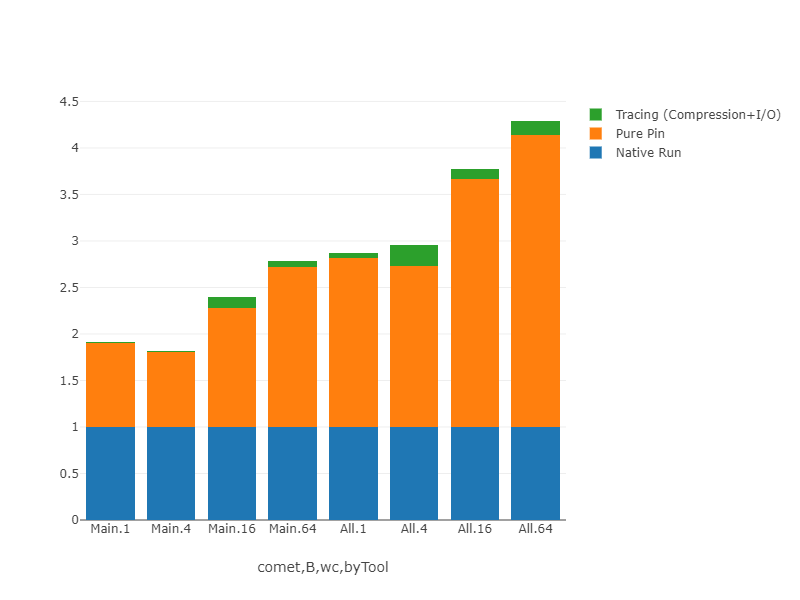
\includegraphics[width=4in]{figs.comet/comet_chartDet_B_wc_byTool_p3_5.png}
\caption{ Input: \textbf{B} - This figure and figure \ref{comet_chartDet_C_wc_byTool_p3_5} shows how much of the overhead of \parlot is caused by \pin and its initialization and how much by that section of \parlot that collects traces and compress them. It seems that overhead added by pure \pin does not scale well and increases with growing number of cores.
}
\label{comet_chartDet_B_wc_byTool_p3_5}
\end{figure}


\begin{figure}[!t]
\centering
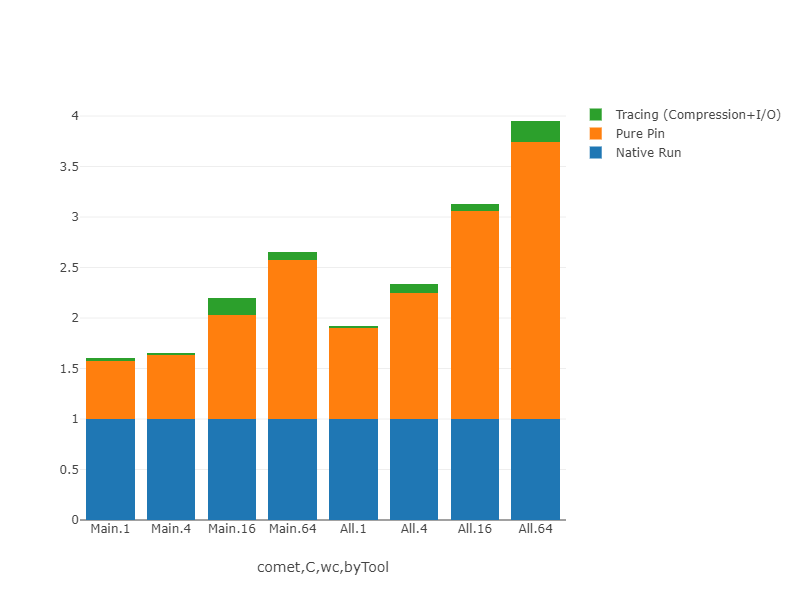
\includegraphics[width=4in]{figs.comet/comet_chartDet_C_wc_byTool_p3_5.png}
\caption{ Input: \textbf{C}
}
\label{comet_chartDet_C_wc_byTool_p3_5}
\end{figure}











\subsection{Compression impact} 
\label{subsec:compact}
\parlot without compression is terrible. (high impact of compression method on performance)
 - Table \ref{comet_wo_det_All_all_B_p3.5}, \ref{comet_wo_det_Main_all_B_p3.5}
   - Fig \ref{comet_chartDet_B_woc_byTool_p3_5}, \ref{comet_chartDet_C_woc_byTool_p3_5}
   
Figures \ref{comet_chartDet_B_wc_byTool_p3_5}, \ref{comet_chartDet_C_wc_byTool_p3_5}, \ref{comet_chartDet_B_woc_byTool_p3_5} and \ref{comet_chartDet_C_woc_byTool_p3_5} clearly show the performance of \parlot and impact of \parlot 's compression mechanism.
	
\begin{itemize}
\item on average, \parlotnc slows down the application execution almost \textbf{2x} more than \parlota. (average overhead of geometric means of all overheads within table  \ref{comet_wo_det_All_all_B_p3.5} for \parlota is \textbf{3.42} and for its coresponding \parlotnc is \textbf{6.62}) . The numbers of \parlotm and input C is following the same pattern. For example, \parlot-nc slows down the application execution almost \textbf{1.66x} more than \parlotm)
\end{itemize}

\begin{figure}[!t]
\centering
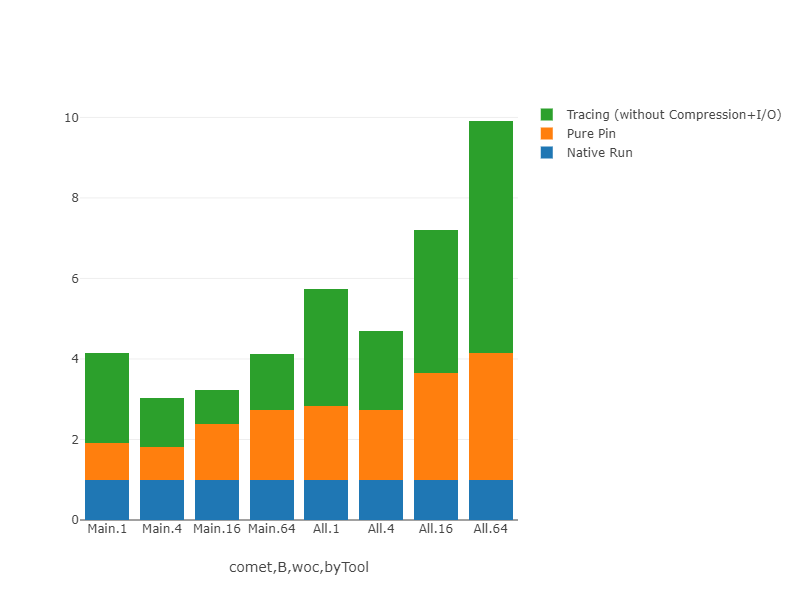
\includegraphics[width=4in]{figs.comet/comet_chartDet_B_woc_byTool_p3_5.png}
\caption{ Input: \textbf{B}- This figure and figure \ref{comet_chartDet_C_woc_byTool_p3_5} shows the impact of \parlot 's data compression.
}
\label{comet_chartDet_B_woc_byTool_p3_5}
\end{figure}

\begin{figure}[!t]
\centering
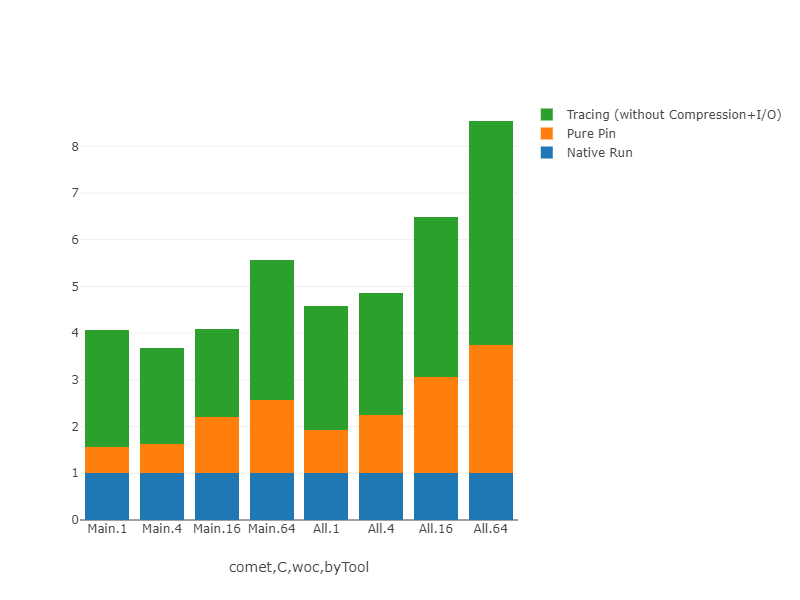
\includegraphics[width=4in]{figs.comet/comet_chartDet_C_woc_byTool_p3_5.png}
\caption{ Input: \textbf{C}
}
\label{comet_chartDet_C_woc_byTool_p3_5}
\end{figure}



